% CHRIS midterm report (ELEC 594): three-page IEEE conference paper.
% Select legacy font encoding before IEEEtran chooses its Times font family.
% This keeps IEEE fonts consistent in Tectonic/XeTeX and pdfLaTeX.
\RequirePackage[T1]{fontenc}
\documentclass[conference,letterpaper]{IEEEtran}
\IEEEoverridecommandlockouts

\usepackage{cite}
\usepackage{amsmath}
\usepackage{graphicx}
\usepackage{booktabs}
\usepackage{url}
\usepackage{pgfplots}
\pgfplotsset{compat=1.18}
\usetikzlibrary{arrows.meta,positioning,calc}
\usepackage[hidelinks]{hyperref}

% Slightly tighter spacing between floats and text to fit three pages.
\setlength{\textfloatsep}{6pt plus 2pt minus 2pt}
% Preserve the font size and margins while fitting the expanded Methods prose.
\linespread{0.98}

\title{Simultaneous AI-Assisted Shared Control for\\Alternative XR Input: A Climbing Testbed}
\author{%
\IEEEauthorblockN{Tongda Yin, Prerna Khanna, Momona Yamagami, and Robert LiKamWa}
\IEEEauthorblockA{Department of Electrical \& Computer Engineering, Rice University,\\
Houston, TX 77005, United States of America}}

% Keep the wide overview on page 1, immediately below the author block.
\makeatletter
\IEEEaftertitletext{%
  \noindent\begin{minipage}{\textwidth}
  \centering
  % Fig. 1: two parallel control paths, read from left to right.
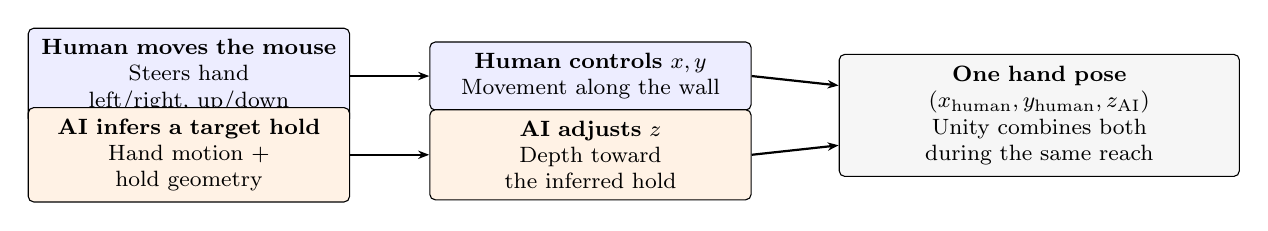
\begin{tikzpicture}[
  font=\footnotesize, >={Stealth[length=4pt]},
  box/.style={draw, rounded corners=2pt, align=center, inner sep=4pt,
    text width=3.8cm, minimum height=0.80cm},
  flow/.style={->, thick}
]
\node[box, fill=blue!7] (human) at (0,0.50)
  {\textbf{Human moves the mouse}\\Steers hand left/right, up/down};
\node[box, fill=orange!10] (ai) at (0,-0.50)
  {\textbf{AI infers a target hold}\\Hand motion + hold geometry};
\node[box, fill=blue!7] (xy) at (5.1,0.50)
  {\textbf{Human controls $x,y$}\\Movement along the wall};
\node[box, fill=orange!10] (z) at (5.1,-0.50)
  {\textbf{AI adjusts $z$}\\Depth toward the inferred hold};
\node[box, text width=4.8cm, minimum height=1.55cm,
  fill=gray!7] (pose) at (10.8,0)
  {\textbf{One hand pose}\\
   $(x_{\rm human},y_{\rm human},z_{\rm AI})$\\
   Unity combines both during the same reach};
\draw[flow] (human) -- (xy);
\draw[flow] (ai) -- (z);
\draw[flow] (xy.east) -- ([yshift=0.38cm]pose.west);
\draw[flow] (z.east) -- ([yshift=-0.38cm]pose.west);
\end{tikzpicture}

  \def\@captype{figure}
  \caption{Two contributions, one reach: the human steers along the wall while
  AI supplies depth. Grabbing and override remain human-controlled.}
  \label{fig:arch}
  \end{minipage}\par\vspace{4pt}}
\makeatother

\begin{document}
\maketitle

\begin{abstract}
We explore simultaneous human--AI shared control to reduce the controls a
person must manage during extended reality (XR) interaction. In a virtual climbing testbed,
the person controls lateral movement and grabbing while heuristic assistance
adjusts depth. Simulations and exploratory headset testing with one developer
reveal tradeoffs among assistance availability, unwanted depth movement, and
additional movement. The developer reported lower depth effort with assistance,
but consistent performance gains remain unestablished. The work demonstrates
how complementary controls can operate during the same action and informs
future adaptation of alternative input devices across XR applications.
Broader workload and accessibility benefits require further evaluation.
\end{abstract}

\begin{IEEEkeywords}
Extended reality, alternative input, shared control, intent inference.
\end{IEEEkeywords}
\section{Introduction}

A mouse supplies planar movement, but reaching a hold in our extended reality
(XR) climbing task also requires depth adjustment. Managing both alongside
grabbing adds controls for the person to coordinate. We ask: \emph{How can a
person and AI control complementary parts of an XR action simultaneously?}
We explore depth assistance while the person steers laterally and grabs,
aiming to reduce simultaneous control demands. AI here means heuristic intent
inference with deterministic control.

Assigning different axes does not determine which hold assistance should
approach or when it should move. Shared-control research connects goal
prediction with assistance arbitration~\cite{losey2018review,dragan2013policy,javdani2018shared};
motion provides pointing cues~\cite{lank2007endpoint}, but misprediction has
costs~\cite{ruiz2010speeding}. Assistance must also respond when human movement
stops. Incorrect assistance can move toward an unintended hold; conservative
assistance can leave depth unfinished.

Using simulations, integration tests, and two headset sessions with one
developer, we compare manual, nearest-hold, and intent-based depth control.
We examine tradeoffs among assistance availability, unwanted depth movement,
and additional human movement. This exploratory study supports the long-term
goal of alternative devices performing common XR actions across applications;
broader workload and accessibility benefits remain unestablished.

\section{Methods}

\subsection{Testbed and Input}
The person remains seated while controlling a virtual climbing task built
in Unity using OpenXR~\cite{openxr} and the XR Interaction
Toolkit~\cite{unity-xri}, connected through Meta Quest Link. The environment
has no falling or momentum; upward movement is capped at 0.25\,m/s, and a
visual vignette is applied~\cite{fernandes2016combating}.

Mouse movement positions the active hand along the wall. Pressing the grab
button attaches the hand to a reachable hold; dragging downward then raises
the virtual body. Releasing the button leaves that hand attached and switches
control to the other hand. An unsuccessful grab preserves existing support.
The grab action uses the left mouse button, with Space used in earlier runs.
E/Q provide manual depth adjustment at 0.15\,m/s.

\subsection{Simultaneous Control and Authority}
The division of control is fixed: the person controls lateral hand movement,
grabbing, and climbing, while assistance adjusts reaching depth. Unity supplies
the Python service with hand positions, the active hand, reaching and gripping
states, and hold geometry. The service uses this information to infer a target
hold and calculate bounded depth adjustments. Images, language, and experimental
target cues are not used for inference.

During each Unity update, human-controlled lateral coordinates $(x,y)$ are
combined with the accepted assisted depth coordinate $z$ to form one hand pose
(Fig.~\ref{fig:arch}). The person can continue moving the mouse while assistance
updates depth. Both therefore contribute during the same reach, even though
the service and Unity update asynchronously.

The person retains control over grabbing and depth override. Grabbing freezes
depth, and pressing E/Q transfers depth control to the person for the remainder
of that reach. Unity rejects stale or invalid assistance updates and handles
interruptions locally; resuming after an interruption requires deliberate
user action.

\subsection{Depth Target and Conditions}
Hand contact uses a 0.04\,m-radius sphere; holds protrude 0.04, 0.08, or
0.12\,m. Assistance targets near-surface contact within a hold's lateral grasp
region, where valid depth exists. Grabs accept a broader overlap interval;
retained depth can permit the next grab without adjustment.

Conditions are \emph{manual} (M; E/Q), \emph{assist-nearest}
(N; the nearest unoccupied hold whose lateral grasp region contains the hand),
and \emph{assist-intent} (I; motion-inferred target). Both assisted conditions
share a depth controller; intent adds the selection rules below.

\begin{figure}[!t]
\centering
% Fig. 2: conditions for moving depth; exact thresholds remain in Methods.
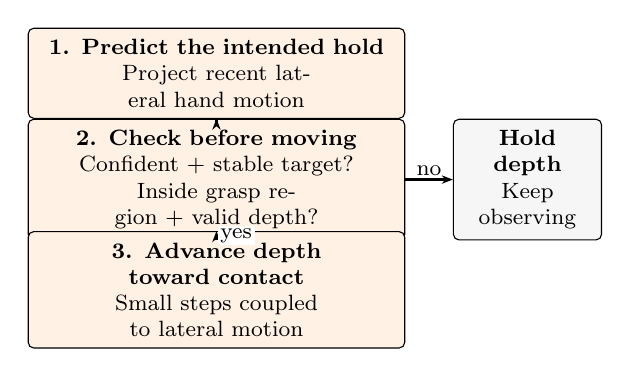
\begin{tikzpicture}[
  font=\footnotesize, >={Stealth[length=4pt]},
  box/.style={draw, rounded corners=2pt, align=center, inner sep=4pt,
    text width=4.50cm},
  flow/.style={->, thick}
]
\node[box, fill=orange!10] (infer) at (0,0)
  {\textbf{1. Predict the intended hold}\\Project recent lateral hand motion};
\node[box, fill=orange!10] (check) at (0,-1.35)
  {\textbf{2. Check before moving}\\Confident + stable target?\\Inside grasp region + valid depth?};
\node[box, fill=orange!10] (move) at (0,-2.75)
  {\textbf{3. Advance depth toward contact}\\Small steps coupled to lateral motion};
\node[draw, rounded corners=2pt, fill=gray!7,
  align=center, text width=1.60cm, inner sep=4pt] (wait) at (3.95,-1.35)
  {\textbf{Hold depth}\\Keep observing};
\draw[flow] (infer) -- (check);
\draw[flow] (check) -- node[right, fill=white, inner sep=1pt] {yes} (move);
\draw[flow] (check) -- node[above, inner sep=1pt] {no} (wait);
\end{tikzpicture}

\caption{Intent-assisted depth (nearest has no confidence gate). Uncertainty holds
depth. After lateral motion stops, the depth budget ends after 150\,ms.}
\label{fig:gate}
\end{figure}

\subsection{Intent Inference and Target Selection}
At 10\,Hz, intent estimates lateral velocity $\vec{v}$ over 250\,ms,
caps speed at 0.3\,m/s, and projects lateral position
$\vec{q}$ to $\hat{\vec{q}}=\vec{q}+(0.5\,\mathrm{s})\vec{v}$.
For unoccupied hold $i$ with lateral centre $\vec{c}_i$ and grasp radius
$r_i$, predicted distance outside its grasp region is
$d_i=\max(0,\|\hat{\vec{q}}-\vec{c}_i\|-r_i)$.
Weights $w_i=\exp(-d_i^2/2\sigma^2)$, with $\sigma=0.08$\,m, and a
``none'' weight of 0.1 are normalized to scores $p_i$.

Selection requires score $p_i\ge0.80$, a 0.25 lead over the runner-up,
and valid grasp geometry and depth, maintained for 200\,ms. A selected target's
score below 0.55 holds depth; persistence for 200\,ms withdraws the target.
Invalid geometry withdraws it immediately (Fig.~\ref{fig:gate}). These rules
follow prediction and arbitration~\cite{dragan2013policy,javdani2015shared};
scores are uncalibrated, and thresholds and hysteresis are design choices.

\subsection{Motion-Coupled Depth Control}
Motion coupling limits both assisted conditions using lateral hand speed.
For eligible target depth $z^*$ and current depth $z_t$, the maximum step
$b_t$ and commanded change are
\begin{equation}
\begin{aligned}
b_t &= \min(0.015\,\mathrm{m},\; 0.6\,\mathrm{m/s}\cdot\Delta t,\; k\tilde v_t\Delta t),\\
\Delta z_t &= \operatorname{sgn}(z^*-z_t)\min(|z^*-z_t|,b_t).
\end{aligned}
\end{equation}
Here $\Delta t$ is the observation interval and $k=1.5$. Effective speed
$\tilde v_t$ uses lateral speed at or above 1\,cm/s, retaining the last such
speed for a 0.15\,s grace period, then zero. Assistance thus continues briefly
after stopping, then holds depth. Steps never exceed
1.5\,cm, within the client's 2\,cm limit. Earlier coupled runs used $k=0.75$
and a 0.15\,m/s cap.

\subsection{Evaluation Design and Measures}
Table~\ref{tab:evidence} summarizes simulations, integration trials, and headset
sessions examining controller tradeoffs, signal delivery, and depth effort,
respectively. The intent sweep served both tuning and evaluation; results
are descriptive.

One developer tested two headset sessions. Each planned one practice
trial/condition and six three-trial blocks: M-N-I-I-N-M, then N-I-M-M-I-N.
Trials required four cued holds; only completed measured trials enter separate
session summaries. Block depth effort used ``Getting the depth right took
effort'' (1: none; 7: a lot). Discomfort $\ge4$ or no rating within 60\,s
stopped the session.

Trial time spans ready to finish. Assistance-state episodes span entry to a
state/target change and are scored against each overlapping reach/cue interval;
wrong-target episodes select a non-cued hold. Headset \emph{engagement coverage}
is the fraction of intervals containing an episode, summarized by the trial
median. States need not produce movement. Wrong-hold travel measures applied
depth changes toward non-cued holds. Simulation coverage averages within-reach
time assisted toward the cue. Causal checks flag unauthorized movement or
direction/cap violations.

Simulated \emph{extra motion} is lateral movement added after lateral arrival
and a depth stall of about 0.3\,s. The headset metric requires a completed cued
reach with a logged coupling hold of at least 0.3\,s followed by resumed
assistance.

\section{Results (Partial)}

\begin{table}[!t]
\caption{Evidence scope. Caps are assisted speeds in m/s; a cell is one condition and setting.}
\label{tab:evidence}
\centering\scriptsize\setlength{\tabcolsep}{3pt}
\begin{tabular}{@{}p{0.25\columnwidth}p{0.36\columnwidth}p{0.31\columnwidth}@{}}
\toprule
Evidence & Configuration & Sample / purpose \\
\midrule
HTTP integration & Uncoupled; cap 0.15 & 9 trials; reliability \\
Intent sweep & Uncoupled; cap 0.15; vary $h,\sigma$ & 400 reaches/setting \\
Coupling test & Off/on; $k=0.75$, cap 0.15 & 400 reaches per cell \\
Speed comparison & $k=0.75$, cap 0.15 vs.\ $k=1.5$, cap 0.6 & 120 reaches per cell \\
Headset sessions & $k=1.5$, cap 0.6 & 1 tester; 15 + 18 completed trials \\
\bottomrule
\end{tabular}
\end{table}

\subsection{Concurrent Control in Integration Runs}
The service and player completed nine scripted HTTP trials without refused or
lost signals, causal-motion violations, or data loss. At 72 frames/s,
observation-to-application latency had medians of 16--40\,ms and a 95th
percentile of 42\,ms.

\begin{figure}[!t]
\centering
% Completed session 2 only: six trials/condition, one developer.
% Read rows 3--5 (manual, nearest, intent) from the verified session extract.
\pgfplotstableread[col sep=comma]{figures/headset-sessions.csv}\headsetdata
\newcommand{\readheadset}[3]{%
  \pgfplotstablegetelem{#1}{#2}\of\headsetdata\let#3\pgfplotsretval}
\readheadset{3}{time_median_s}{\manualTime}
\readheadset{4}{time_median_s}{\nearestTime}
\readheadset{5}{time_median_s}{\intentTime}
\readheadset{4}{false_assist_episodes_total}{\nearestEpisodes}
\readheadset{5}{false_assist_episodes_total}{\intentEpisodes}
\readheadset{3}{depth_effort_ratings}{\manualEffort}
\readheadset{4}{depth_effort_ratings}{\nearestEffort}
\readheadset{5}{depth_effort_ratings}{\intentEffort}
\def\splitratings#1;#2\relax{\def\firstRating{#1}\def\secondRating{#2}}
{\footnotesize\textbf{Session 2: one developer}\par}\vspace{3pt}
\begin{tikzpicture}
\pgfplotsset{headsetpanel/.style={
  scale only axis, height=2.30cm, font=\footnotesize,
  ymin=-0.90, ymax=2.55, ytick={0,1,2},
  axis x line*=bottom, axis y line*=left,
  tick align=outside, xmajorgrids, grid style={gray!20},
  title style={align=center, font=\footnotesize},
  clip=false,
}, timepoint/.style={only marks, mark=|, mark size=4pt, ultra thick}}
\begin{axis}[headsetpanel, name=timeplot, width=2.10cm,
  xmin=0, xmax=21, xtick={0,10,20},
  yticklabels={Intent,Nearest,Manual},
  title={\textbf{Trial time}\\Seconds}]
% The trial CSV is ordered manual (0--5), nearest (6--11), intent (12--17).
\addplot[only marks, mark=o, mark size=1.4pt, gray!80!black,
  restrict expr to domain={\coordindex}{0:5}]
  table[col sep=comma, x=time_s, y=plot_y] {figures/headset-session2-trials.csv};
\addplot[only marks, mark=o, mark size=1.4pt, blue!65!black,
  restrict expr to domain={\coordindex}{6:11}]
  table[col sep=comma, x=time_s, y=plot_y] {figures/headset-session2-trials.csv};
\addplot[only marks, mark=o, mark size=1.4pt, orange!85!black,
  restrict expr to domain={\coordindex}{12:17}]
  table[col sep=comma, x=time_s, y=plot_y] {figures/headset-session2-trials.csv};
\addplot[timepoint, gray!80!black] coordinates
  {(\manualTime,2)};
\addplot[timepoint, blue!65!black] coordinates
  {(\nearestTime,1)};
\addplot[timepoint, orange!85!black] coordinates
  {(\intentTime,0)};
\node[font=\scriptsize\bfseries, anchor=north, inner sep=0.5pt]
  at (axis cs:\manualTime,1.65) {\pgfmathprintnumber[fixed,precision=1]{\manualTime}};
\node[font=\scriptsize\bfseries, anchor=north, inner sep=0.5pt]
  at (axis cs:\nearestTime,0.65) {\pgfmathprintnumber[fixed,precision=1]{\nearestTime}};
\node[font=\scriptsize\bfseries, anchor=north, inner sep=0.5pt]
  at (axis cs:\intentTime,-0.35) {\pgfmathprintnumber[fixed,precision=1]{\intentTime}};
\end{axis}
\begin{axis}[headsetpanel, name=effortplot, width=1.55cm,
  at={(timeplot.south east)}, anchor=south west, xshift=0.55cm,
  xmin=0.5, xmax=7.5, xtick={1,4,7}, yticklabels={,,},
  title={\textbf{Depth effort}\\Rating (1--7)}]
\expandafter\splitratings\manualEffort\relax
\addplot[only marks, mark=*, mark size=2pt, gray!80!black]
  coordinates {(\firstRating,2.10) (\secondRating,1.90)};
\expandafter\splitratings\nearestEffort\relax
\addplot[only marks, mark=*, mark size=2pt, blue!65!black]
  coordinates {(\firstRating,1.10) (\secondRating,0.90)};
\expandafter\splitratings\intentEffort\relax
\addplot[only marks, mark=*, mark size=2pt, orange!85!black]
  coordinates {(\firstRating,0.10) (\secondRating,-0.10)};
\node[font=\scriptsize, align=center, anchor=north, yshift=-15pt]
  at (rel axis cs:0.5,0) {1 = none\\7 = a lot};
\end{axis}
\begin{axis}[headsetpanel, width=1.80cm,
  at={(effortplot.south east)}, anchor=south west, xshift=0.55cm,
  xmin=0, xmax=12, xtick={0,5,10}, yticklabels={,,},
  title={\textbf{Wrong-target}\\State episodes},
  xbar, bar width=7pt, bar shift=0pt,
  nodes near coords, point meta=x,
  every node near coord/.append style={font=\scriptsize, text=black}]
\addplot[fill=blue!30, draw=blue!65!black] coordinates {(\nearestEpisodes,1)};
\addplot[fill=orange!40, draw=orange!85!black] coordinates {(\intentEpisodes,0)};
\node[font=\scriptsize] at (axis cs:5,2) {N/A};
\node[font=\scriptsize, align=center, anchor=north, yshift=-15pt]
  at (rel axis cs:0.5,0) {Engagement coverage\\Nearest 100\%; Intent 75\%};
\end{axis}
\end{tikzpicture}

\caption{Complete session 2; six trials/condition. Time: trials (circles),
medians (bars and labels). Effort: two block ratings. Marks are offset vertically.
Episodes are state-based totals; manual has no AI. Engagement is median trial
coverage. Lower counts accompany less engagement.}
\label{fig:headset}
\end{figure}

\subsection{Intent Inference and Assistance Availability}
Compared with nearest, the chosen setting ($h = 0.5$, $\sigma = 0.08$) about
halved false-assist time toward distractor P (0.511 vs.\ 1.006\,s per reach crossing P).
The cost was lower coverage (0.327 vs.\ 0.387) and a
longer median reach-start-to-first-correct-assistance time (2.01 vs.\ 1.67\,s;
among reaches receiving correct assistance). These parameters were selected
on the same sweep; the comparison is exploratory.

\subsection{Coordinating Human Motion and Assisted Depth}
During 1\,s hovers over P (75 per condition), depth travel \emph{after} the
0.15\,s grace was 110.5\,mm (nearest) and 123.7\,mm (intent) without coupling,
and zero with it. Coupled nearest still moved 21.7\,mm during the grace.
In 400 reaches/condition, coupling required extra scripted movement on
32\% (nearest) and 77\% (intent), versus 0\% and 9\% without coupling.

In the separate speed comparison, raising $k$ and the cap reduced extra-motion
rates from 30\% to 17\% (nearest) and 72\% to 53\% (intent).
Mean wrong-hold travel rose from 49.7 to 83.1\,mm per reach (nearest) and
18.2 to 33.1\,mm (intent): faster recovery increased misdirected travel.

\subsection{Headset Testing (Developer)}
After a pilot stopped at discomfort 4, interrupted session 1 completed
15 measured trials (M: 3, N: 6, I: 6), excluding three incomplete attempts.
Session 2 completed 18/18 (six/condition) plus three practice trials, without
data loss, causal-motion violations, or no-signal pauses. All measured
completions used the final configuration.

Median trial times (M/N/I) were 36.5/11.7/13.4\,s in session 1 and
11.2/9.8/11.4\,s in session 2 (Fig.~\ref{fig:headset}). Wrong-target assistance episodes (N/I,
session totals) were 21/7 and 9/2, respectively. In session 2, median
wrong-hold depth travel was 39.6/0\,mm per trial, but maximum single-reach
travel was 185.8/93.3\,mm. Extra motion was required on 0/24 nearest and
1/24 intent cued reaches.

The developer reported lower effort with assistance (1--2 versus 7),
discomfort 1, no clear nearest/intent difference, and no stereo artifacts
after fixes.

\section{Discussion (Partial)}

Concurrent lateral and depth control lets both contribute during one reach.
Assistance handles depth but must select a hold and time its movement to
limit motion toward unintended targets.

Intent's fewer wrong-target episodes accompanied lower engagement, not
necessarily better inference. Coupling stopped depth after the grace period
but could leave it unfinished. Higher gain and caps reduced additional
scripted movement while increasing wrong-hold travel.

The developer reported lower depth effort, but session 2 showed little timing
advantage. Retained depth and overlap-based grabs allowed 8/24 manual reaches
without depth input. Practice, order, and software changes limit comparison;
perceptible intent benefits remain unestablished.

Intent required extra motion on 53\% of simulated reaches but 1/24 in session 2.
Different movement policies and scoring prevent direct comparison or prediction
of a human rate.

Evidence comes from one developer and simulations sharing tuning and evaluation
data. Gain and cap changed together; manual and assisted caps differed.
Wrong-hold travel measures disagreement, not harm; control authority does not
establish perceived agency. Accessibility benefits and transfer to other XR
actions remain untested.

\section{Conclusion}
This climbing testbed demonstrates simultaneous shared control: the person
controls lateral movement and grabbing while heuristic assistance adjusts
depth. The experiments reveal a tradeoff between providing assistance,
limiting unwanted depth movement, and requiring additional movement.
One developer reported lower depth effort, but consistent performance gains
and benefits of intent over nearest assistance remain unestablished.
Enabling alternative devices to perform common XR actions across applications
remains the long-term goal.

\section*{Acknowledgements}
Tongda Yin thanks co-authors Prerna Khanna, Momona Yamagami, and Robert LiKamWa
for their supervision and mentorship, and the ELEC 594
course staff for their feedback.

\section*{CRediT Author Statement}
\textbf{Tongda Yin:} Conceptualization, Methodology, Software, Validation,
Investigation, Data curation, Visualization, Writing -- original draft,
Writing -- review \& editing.
\textbf{Prerna Khanna, Momona Yamagami, and Robert LiKamWa:}
Supervision and mentorship.


\bibliographystyle{IEEEtran}
\bibliography{references}

\end{document}
